
\chapter{实验结果}
\label{chap:result}

我们比较了上一节中所提到的方法的预测性能,并列出了表4 (AUC)、精度(Prec)、召回(Rec)和 F1 测量(F1)。并结合两个实际的案例来探索其应用价值。
请见表




\section{参数调整}\label{sec:anly}

GHSOM中的超参数主要有初始映像图大小、广度参数和深度参数这三个。
通过实际的数据,观察不同的初始映像图大小会在多大程度上影响神经网络的学习。这里基于不同初始映像图大小进行实验。结果如图\ref{fig:initialization}所示。

\begin{figure}[!htbp]
    \centering
    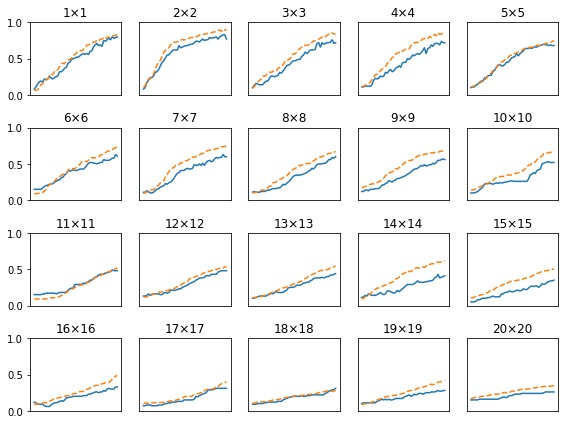
\includegraphics[width=0.8\textwidth]{sominit}
    \caption{实线是验证数据的识别精度,虚线是训练数据的识别精度}
    \label{fig:initialization}
\end{figure}


从图\ref{fig:initialization}中,按识别精度从高到低的顺序排列了验证数据的学习的变化。从图中可知,直到“4×4”左右,学习进行得都很顺利。因此,我们来 观察一下“4×4”之前的超参数的值(学习率),结果如下表\ref{tab:init}所示。从这个结果可以看出,学习率在 0.001 到 0.01时,学习可以顺利进行。


\begin{table}[!htbp]
    \caption{实验结果}
    \label{tab:init}
    \centering
    \footnotesize% fontsize
    \setlength{\tabcolsep}{4pt}% column separation
    \begin{tabular}{l*{5}{c}r}
        size       & val acc  & lr  \\
        \hline
        1×1        & 0.83     & 0.0092  \\
        2×2        & 0.78     & 0.00956 \\
        3×3        & 0.77     & 0.00571 \\
        4×4        & 0.74     & 0.00626 \\
    \end{tabular}
\end{table}

\section{算法应用}
本章节将从舆情监控和广告投放两方面的案例进行分析。

\subsection{舆情监控}
在这一部分中,将本文算法得出的结果与微博名下的大数据监控平台微热点的相关分析结果做比较。微热点将微博话题简单的分成了政治、经济、法治、教育、商业、民生、医疗、交通、文娱和体育十大板块。

我们根据系统架构所提出的方法,提取2019年3月21日下午14时48分左右江苏盐城爆炸事件相关微博,该事件至论文完成时已经累积2.6亿次阅读,属于突发事件。部分微博机构、用户的影响力占比如下表所示。





\subsection{广告投放}

某著名微博营销网站采用的用户投放报价方式,是基于传统的转发、评论、点赞,如图所示..

